\begin{figure*}[!ht]
  \centering
  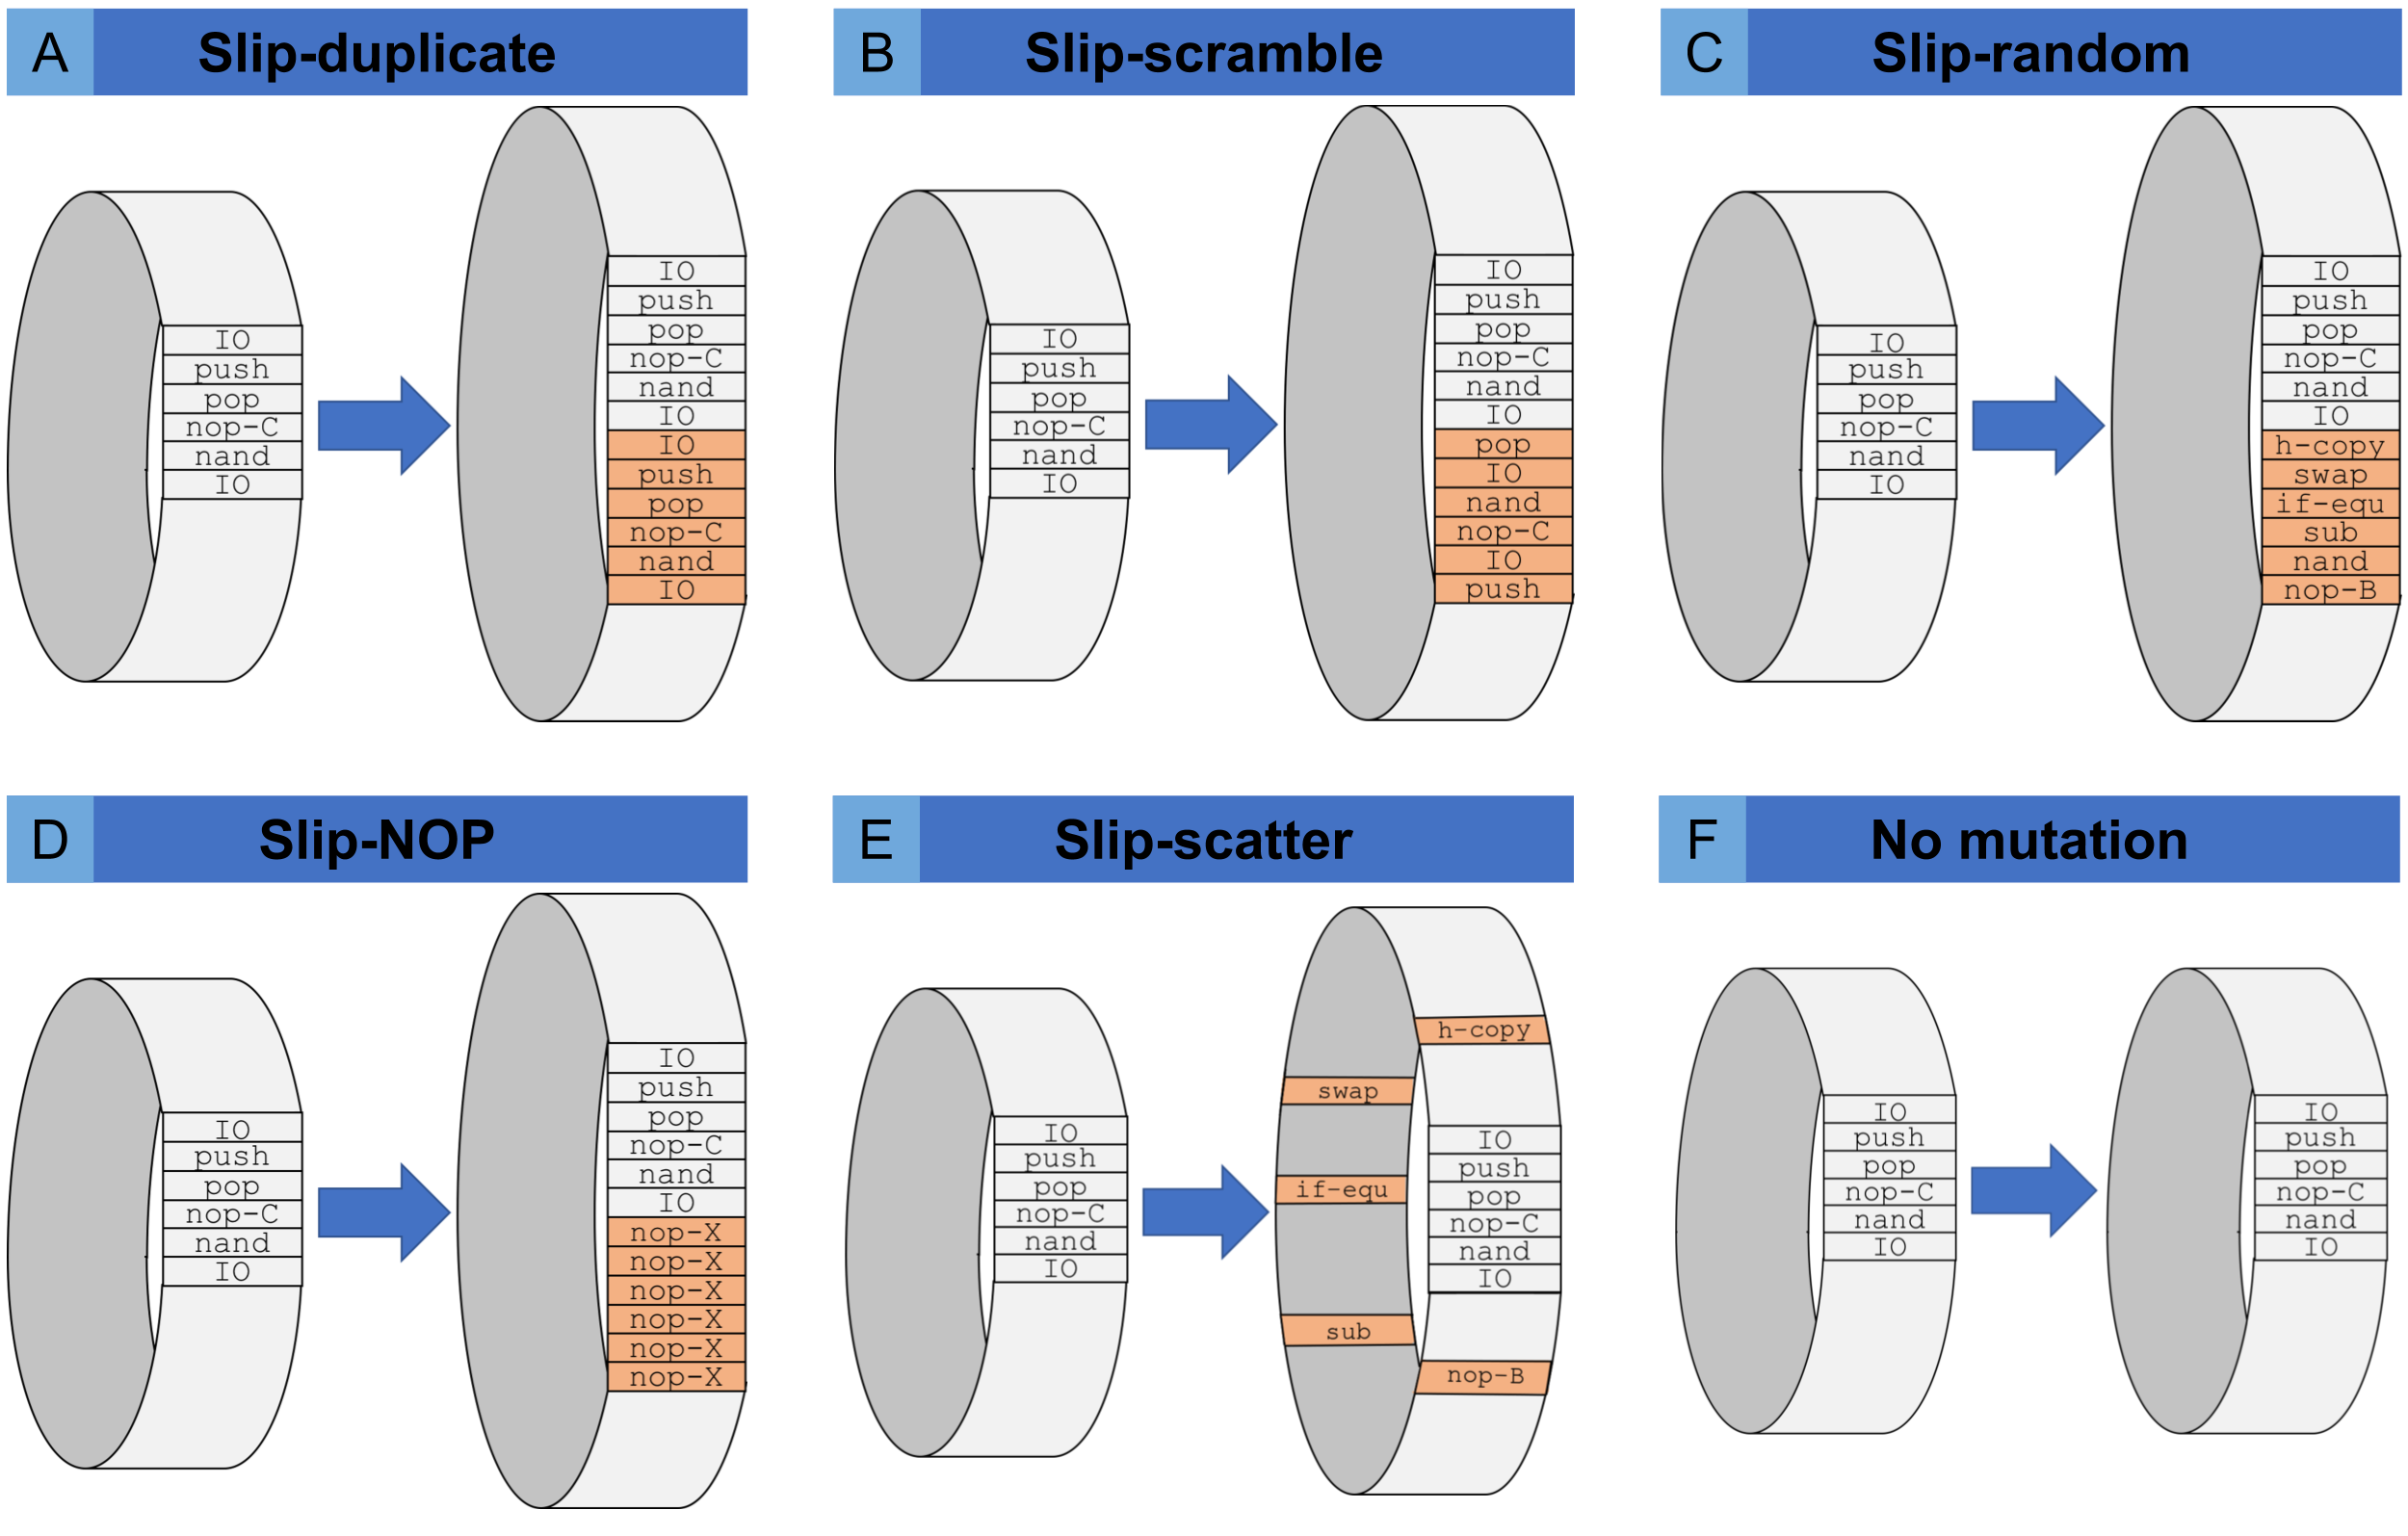
\includegraphics[width=\textwidth]{imgs/slip_mutation_variants.png}
   % 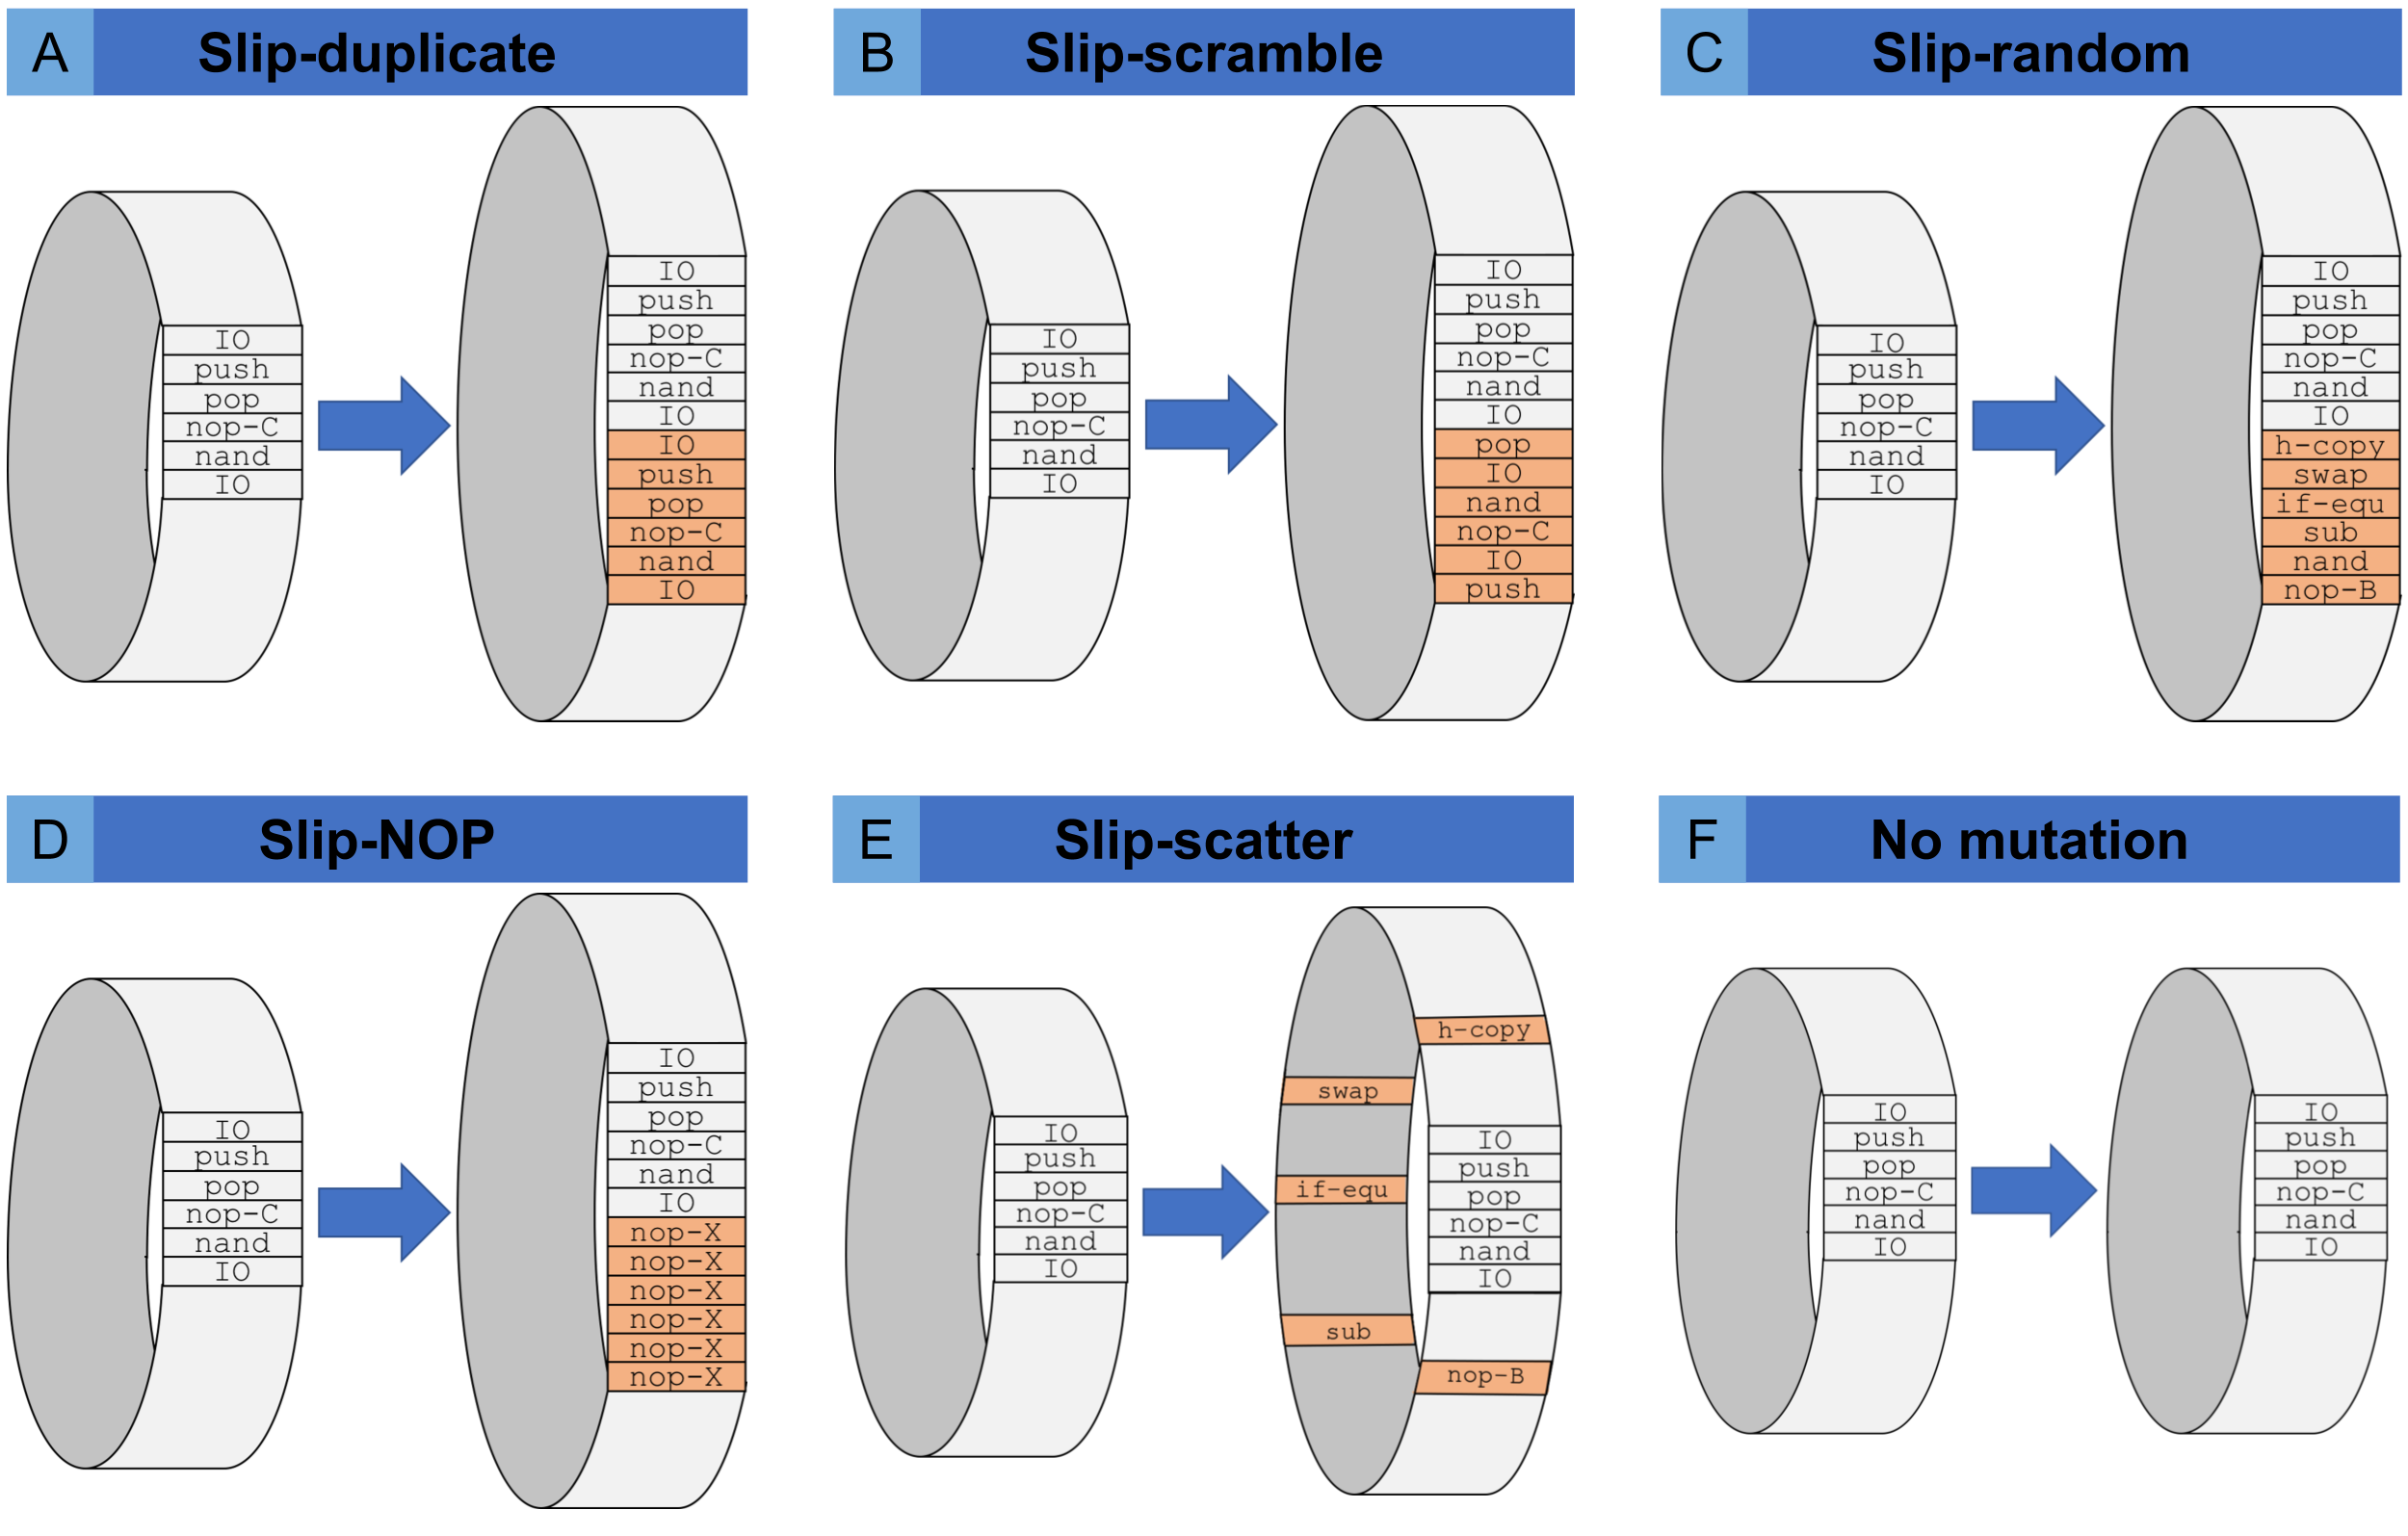
\includegraphics[height=0.4\textheight]{imgs/slip_mutation_variants.png}
    \caption{\small Descriptions and visual examples of how each of our slip mutation operator handles insertions. A) Slip-duplicate: The inserted segment is an exact duplicate of the target segment and is inserted directly after the target segment. B) Slip-scramble: The inserted segment is a shuffled duplicate of the target segment and is inserted directly after the target segment. C) Slip-random: The inserted segment consists of random instructions and is inserted directly after the target segment. D) Slip-NOP: The inserted segment consists of nop-X instructions (a no operation instruction in Avida) and is inserted directly after the target segment. E) Slip-scatter:  The inserted segment consists of random instructions and is broken up and inserted into random locations in the genome. F) For comparison, we include an example with no mutation. }
    \label{fig:slip_mut_variants}
\end{figure*}
